\documentclass[10pt,a4paper]{article}
\usepackage[utf8]{inputenc}
\usepackage{amsmath}
\usepackage{amsfonts}
\usepackage{amssymb}
\usepackage[top=2cm, bottom=2cm, left=2cm, right=2cm]{geometry}
\usepackage{graphicx}
\author{Jean Destribois - 21602062}
\title{Calcul Sécurisé - Contrôle Continu}
\date{Avril 2020}

\begin{document}
\maketitle

\section{Question 1}
Injecter une faute sur $R_{15}$ dans le DES revient à faire un $XOR$ (ou exclusif) d'une certaine valeur $e$ sur $R_{15}$. Comme on a $R_{16} = R_{15}$, l'attaque revient à faire également un $XOR$ de la même valeur $e$ sur $R_{16}$. Concernant $L_{16}$, l'attaque revient à faire un $XOR$ d'une valeur $e'$ sur $L_{16}$ tel que :
\[L_{16} \oplus e' = L_{15} \oplus F(R_{15} \oplus e,\ K_{16})\]
\begin{center}où $\oplus$ correspond au XOR et $F$ une fonction décrite dans le DES.\end{center}
On appelle $L'_{16}$ la partie gauche et $R'_{16}$ la partie droite du DES fauté au 16ème tour tels que : 
\[L'_{16} = L_{16} \oplus e' = L_{15} \oplus F(R_{15} \oplus e,\  K_{16})\]
\begin{center}et\end{center}
\[R'_{16} = R_{16} \oplus e = R_{15} \oplus e\]
Voir les deux ces deux schémas \ref{schema 1} \ref{schema 2} en annexe.

\subsection{Trouver $e$}
On cherche dans un premier temps à retrouver $e$. Pour cela, on considérera qu'on a un chiffré $C$ d'un message $M$ et un chiffré fauté $C'$ du même message $M$. Les deux ayant été chiffrés par une même clé $K$.
On a :
\[C = IP^{-1}(L_{16}\ ||\ R_{16})\]
\[C' = IP^{-1}(L'_{16}\ ||\ R'_{16})\]
\begin{center}où $||$ est l'opération de concaténation et $IP^{-1}$ la fonction inverse de la permutation $IP$.\end{center}
Comme la fonction $IP$ est connue et bijective. On est capable de calculer :
\[IP(C) = L_{16}\ ||\ R_{16}\]
\[IP(C') = L'_{16}\ ||\ R'_{16}\]
On sait que $L_{16}$ et $R_{16}$ (ainsi que $L'_{16}$ et $R'_{16}$) sont de la même taille. On est donc capable à ce stade de séparer en deux le résultat et obtenir $L_{16}$ et $R_{16}$ (ainsi que $L'_{16}$ et $R'_{16}$). On applique ensuite un $XOR$ entre $R_{16}$ et $R'_{16}$ :
\[R_{16} \oplus R'_{16} = R_{16} \oplus R_{16} \oplus e=e\]
Ainsi nous avons obtenu $e$.

\subsection{Trouver $K_{16}$}
Maintenant que nous avons obtenu ces valeurs, nous cherchons la clé $K_{16}$ utilisée dans la fonction $F$.
On rappelle que la fonction $F$ est est défini ainsi pour $R_{15}$ et $K_{16}$ en valeur d'entrée :
\[F(R_{15},\ K_{16}) = P(S(K_{16}\oplus E(R_{15})))\]
\begin{itemize}
\item $P$ une fonction de permutation bijective
\item $S$ une fonction composée de 8 "S-Box" appliquées à chaque blocs de 6 bits d'un mot de 48 bits et donnant en sortie 4 bits (et donc formant un mot de 32 bits)
\item $E$ une fonction d'expansion prenant en entrée un mot de 32 bits et donnant en sortie un mot de 48 bits.
\end{itemize}
Pour trouver $K_{16}$, il est nécessaire d'avoir en sa possession plusieurs chiffrés $C'$ fautés de manière différente. On applique ce qui a été décrit précédemment pour trouver chaque $e$ correspondants à chaque chiffrés $C'$. On rappelle qu'on a d'après la définition de la fonction $F$ :
\[L'_{16} = L_{15} \oplus P(S(K_{16} \oplus E(R_{15} \oplus e)))\]
On calcul alors pour chaque $L'_{16}$ :
\[L_{16} \oplus L'_{16} = L_{15} \oplus P(S(K_{16} \oplus E(R_{15}))) \oplus L_{15} \oplus P(S(K_{16} \oplus E(R_{15} \oplus e)))\]
Les $L_{15}$ s'annulent, on a alors :
\[L_{16} \oplus L'_{16} = P(S(K_{16} \oplus E(R_{15}))) \oplus P(S(K_{16} \oplus E(R_{15} \oplus e)))\]
On peut ensuite appliquer la fonction de permutation inverse $P^{-1}$ :
\[P^{-1}(L_{16} \oplus L'_{16}) = S(K_{16} \oplus E(R_{15})) \oplus S(K_{16} \oplus E(R_{15} \oplus e))\]
En calculant $E(e)$, on pourra savoir sur quelles S-Box $e$ provoque une modification (grâce aux bits à 1). On travaillera ensuite seulement sur ces $S_{i}$ (correspondant à la S-Box d'indice $i$). On effectuera une recherche exhaustive  sur les 6 bits de clé de $K_{16}$ en entrée des $S_{i}$ correspondantes : 
\[S_{i}(k_{j} \oplus E(R_{15})_{i}) \oplus S_{i}(k_{j} \oplus E(R_{15} \oplus e)_{i}) \stackrel{?}{=} P^{-1}(L_{16} \oplus L'_{16})_{i}\]
\begin{center}Où l'indice $i$ correspond à l'indice de la S-Box concernée et à la partie d'un mot correspondant également à la S-Box et $k_{j}$ correspond au 6 bits de clé qu'on teste.\end{center}
On garde toutes les $k_{j}$ vérifiant l'égalité précédente. On obtient ainsi un ensemble de partie de clés possible pour chaque S-Box. On choisit la partie de clé présente pour tous les $C'$ et en concaténant dans l'ordre chaque parties de clé trouvées dans le bon ordre, on obtient $K_{16}$.

\subsection{Trouver $K$}
La dernière étape est maintenant de trouver la clé $K$ (de 56 bits) qui a permis de générer la clé $K_{16}$ (de 48 bits). Voir le schéma \ref{schema 3} en annexe pour la génération de ces clés.
\\La fonction $PC2$ est une fonction d'extraction prenant en entrée un mot 56 bits et donnant en sortie un mot de 48 bits. Dans le cas de $K_{16}$ on cherche donc à retrouver $x = C_{16}||D_{16}$ (de 28 bits chacun) tels que $PC2(x) =  K_{16}$. On est capable de retrouver retrouver 48 bits de $x$ à partir de $K_{16}$ cependant 8 des bits de $x$ seront inconnus (ceux à la position 9, 18, 22, 25, 35, 38, 43, 54). Il sera donc nécessaire de faire une recherche exhaustive sur ces 8 bits de $x$.
\\Pour chacun des $x$ supposés, il faudra remonter jusqu'à $PC1(K) = C_{0}||D_{0}$. A partir de $PC1(K)$ l'algorithme de génération de clé effectue 28 rotation sur $C_{0}$ et $D_{0}$, comme ces deux derniers ont une taille de 28 bits, cela revient à faire un tour complet sur eux-mêmes et donc :
\[C_{0} = C_{16}\]
\[D_{0} = D_{16}\]
et donc :
\[x = PC1(K)\]
Comme on connait $PC1()$, et qu'on est capable de retrouver $K$ à partir de $x$ tels que $PC1(K) = x$ en appliquant les bits de parité comme décrit dans le DES, il suffit de calculer $PC1^{-1}(x)$ et appliquer les bits de parité pour trouver la clé $K$. On teste ensuite pour chaque $x$ supposés, si pour la clé $K$ obtenue, le chiffré du message $M$ donne le bon chiffré $C$. Ainsi on aura obtenu la bonne clé $K$.

\subsection{Complexité}
Pour la complexité du procédé décrit précédemment, il faut prendre en compte la recherche exhaustive de la clé $K_{16}$ et la recherche exhaustive de $x$ nous permettant de trouver $K$ :
\begin{itemize}
\item Pour $K_{16}$ : $2^{6}$ choix pour les 8 S-Box. Et 32 chiffrés fautés dans notre cas à tester. Donc au total, on obtient une complexité de $\mathcal{O}(2^{6}\times 8 \times 32) = \mathcal{O}(2^{14})$.
\item Pour $K$ : 8 bits inconnus, on obtient donc une complexité de $\mathcal{O}(2^{8})$.
\end{itemize}
On a donc au total une complexité de $\mathcal{O}(2^{14} + 2^{8})$.

\section{Programme}
\subsection{Langage de programmation}
J'ai choisi pour implémenter cette attaque d'utiliser le langage C : langage très procédurale et bas niveau correspondant bien au type de l'attaque.

\subsection{Exécution}
Pour exécuter le programme, j'ai éditer un fichier \textit{Makefile} permettant d'automatiser la compilation et l'exécution : il suffit de se placer dans le dossier \textit{programme} du projet et d'entrer la commande \textit{make}. Le programme effectuera l'attaque et affichera ensuite dans le terminal la valeur de la clé $K_{16}$ et la valeur de $K$. 

\subsection{Question 2}
Pour implémenter cette attaque il a d'abord été nécessaire que je développe un programme effectuant le chiffrement DES entièrement pour me permettre de faire la recherche exhaustive de la clé $K$ à partir de $K_{16}$. J'ai donc créé un fichier \textit{DES.c} avec son header \textit{DES.h} contenant toutes les constantes du DES (S-box, tables de permutation et d'expansion) et la définition de 7 fonctions.

Ensuite j'ai créé un fichier \textit{attaque.c} et son header \textit{attaque.h} contenant les tables de permutation inverse que le DES ne contient pas déjà (pour la table $PC2$ 8 bits restent inconnus), définissant une structure pour l'attaque, une structure de liste chainée et définissant 8 fonctions.

Ce programme va d'abord lire les données de l'attaque stockées dans le dossier \textit{donnees$\_$attaque} et les stocker dans la structure de donnée \textit{struct attaque}. Ensuite il effectue la recherche de $K_{16}$ de la manière décrite dans la partie 1.2. Il va stocker toutes les parties de clé possible dans un tableau de listes chainées (comme on ne connait pas le nombre de partie clés qui fonctionnent pour un chiffré fauté et pour une S-Box). Il va ensuite, pour chaque S-Box, sélectionner les parties de clés présentes dans les listes chainées pour tous les chiffrés dont la liste est non nulle. On obtient ainsi, en concaténant ces parties de clé, la clé $K_{16}$ qui est en hexadécimal est : $BC\ D4\ D5\ 33\ B9\ D1$.

\subsection{Question 3}
Il va ensuite faire la recherche de $K$ de la manière décrite dans la partie 1.3. 
On obtient donc la clé $K$ qui est en hexadécimal avec les bits de parité : $B5\ CD\ D7\ 93\ 2F\ 63\ F7\ C5$.

\section{Question 4}
\subsection{Attaque par fautes sur $R_{14}$}
Injecter une faute sur $R_{14}$ dans le DES revient à faire un XOR d'une certaine valeur $e$ sur $R_{14}$. En reprenant le même schéma du DES et les même notation que pour les questions précédentes, on a :
\[R'_{16} = R'_{15} = L_{14} \oplus F(R_{14} \oplus e,\ K_{15})\]
\begin{center}et\end{center}
\[L'_{16} = L'_{15} \oplus F(R'_{15},\ K_{16}) = R_{14} \oplus e \oplus F(R'_{15},\ K_{16})\]
De plus on a :
\[R'_{16} \oplus R_{16} = L_{14} \oplus F(R_{14} \oplus e, K_{15}) \oplus L_{14} \oplus F(R_{14}, K_{15})\]
\[R'_{16} \oplus R_{16} = F(R_{14} \oplus e, K_{15}) \oplus F(R_{14}, K_{15})\]
\[P^{-1}(R'_{16} \oplus R_{16}) = S(K_{15} \oplus E(R_{14} \oplus e)) \oplus S(K_{15} \oplus E(R_{14}))\]
Cela ressemble beaucoup aux éléments que nous détenions pour l'attaque par injection de fautes sur $R_{15}$. Il faudrait connaître $R_{14}$ et $R'_{14}$ pour pouvoir effectuer la même attaque, cependant nous ne les connaissons pas. Nous allons donc procéder de la même manière que ce qui est décrit dans la partie 1.2 sauf qu'il sera également nécessaire avant de faire une recherche exhaustive sur chacun des 4 bits de $R_{14}$ et $R'_{14}$ (je n'ai malheureusement pas réussi à trouver de quelle manière on pouvait tester les $R_{14}$ et $R'_{14}$ pour cette recherche exhaustive). De plus on ne connait pas $e$ donc on n'est pas capable d'obtenir $R'_{14}$ à partir de $R_{14}$. Cependant, si on considère que la faute $e$ ne modifie $R_{14}$ que sur un seul bit (comme c'était le cas pour les données de l'énoncé de ce contrôle), alors pour chaque 4 bits de $R_{14}$, il faudra tester 4 possibilités différentes pour $R'_{14}$.\\
On a alors :
\begin{itemize}
\item 32 chiffrés fautés à tester dans notre cas.
\item 8 S-Box à tester.
\item $2^{4}$ valeurs de $R_{14}$ à tester pour chaque partie de $K_{15}$ qu'on teste.
\item 4 valeurs de $R'_{14}$ à tester pour chaque $R_{14}$ qu'on teste.
\end{itemize}
On fini avec une complexité en $\mathcal{O}(32 \times 8 \times 2^{4} \times 4) = \mathcal{O}(2^{14})$.\\
Suite à cela, il faudra faire la recherche exhaustive de $K_{15}$ comme dans la partie 1.2 pour chacun des $R_{14}$ et $R'_{14}$ possibles qu'on a trouvés. Cette recherche est d'une complexité en $\mathcal{O}(2^{14})$. Ce qui nous donne au total, pour la recherche de $K_{15}$ une complexité en $\mathcal{O}(2^{14} \times 2^{14}) = \mathcal{O}(2^{28})$

Une fois $K_{15}$ obtenu, retrouver $K$ revient à faire la même chose que ce qui est décrit dans la partie 1.3, cependant il sera nécessaire de penser à rajouter une rotation circulaire vers la droite sur $C_{15}$ et $D_{15}$ pour retrouver $C_{0}$ et $D_{0}$. Cette recherche de $K$ se fera donc avec une complexité en $\mathcal{O}(2^{8})$ comme dans la partie 1.3.

Au total cette attaque par fautes sur $R_{14}$ est d'une complexité en $\mathcal{O}(2^{28} + 2^{8})$.

\subsection{Attaque par fautes sur $R_{i}$}
Pour une attaque par fautes sur $R_{13}$ le principe est le même que ce qui a été décrit précédemment : il faudra faire une supposition sur $R_{14}$ et $R'_{14}$ puis sur $R_{13}$ et $R'_{13}$. Cela entraine donc une complexité en $\mathcal{O}(2^{14})$ pour la recherche de $R_{14}$ et $R'_{14}$ puis une complexité en $\mathcal{O}(2^{14})$ pour la recherche de $R_{13}$ et $R'_{13}$ et enfin une complexité en $\mathcal{O}(2^{14})$ pour la recherche de $K_{14}$. La recherche de $K$ reste la même à condition de prendre en compte à chaque fois le bon nombre de rotation circulaire sur $C_{14}$ et $D_{14}$. On aura donc une recherche d'une complexité en $\mathcal{O}(2^{42} + 2^{8})$.\\
Cette méthode se répètera de la même manière pour chaque attaque par fautes sur $R_{i}$ et on obtiendra une complexité pour une attaque par fautes sur $R_{10}$ en $\mathcal{O}(2^{84} + 2^{8})$. Cette complexité est trop élevé pour la puissance de calcul des ordinateurs actuels. On en déduit que cette attaque n'est plus réaliste à partir de $R_{10}$.

\section{Question 5}
Une contre-mesure possible pour cette attaque serait de protéger physiquement le support sur lequel le DES est implémenté : on pourrait, par exemple, poser une matière sur les composants électroniques qui protégerait une injection de fautes par l'utilisation d'un laser. Cette matière pourrait endommager les circuits électronique si quelqu'un tenterait d'enlever cette matière. Cela n'est pas toujours faisable car certains appareils on besoin d'un contact extérieur pour fonctionner (par exemple une carte bancaire).\\
Une autre contre-mesure possible serait de protéger dans l'implémentation même. On pourrait par exemple refaire le calcul du chiffrement une deuxième fois (ou plus) et comparer le résultat avec ce qui a été obtenu précédemment. Si le résultat n'est pas le même, alors il a été fauté. Cette contre-mesure rallonge le temps de calcul autant de fois qu'on refait le calcul. Cela peut être un problème pour certaines utilisations.





\appendix
\newpage
\section{Annexes}
\subsection{Schéma de DES sans attaque par fautes}
\label{schema 1}
\vspace*{\stretch{1}} \begin{center}
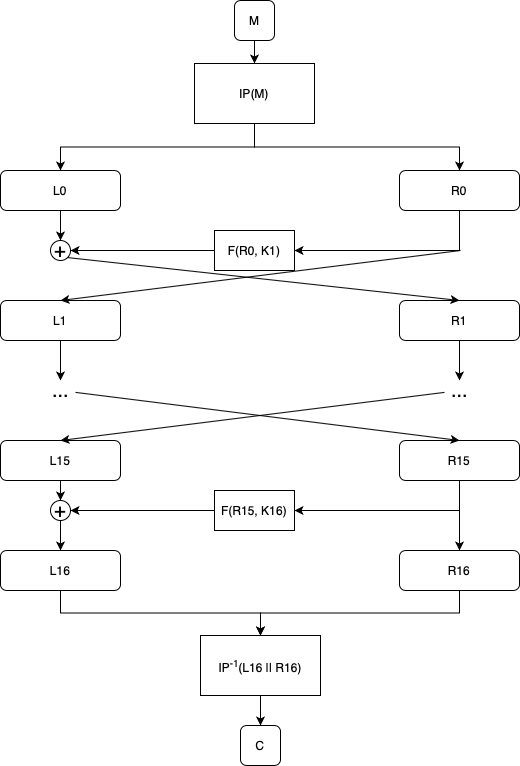
\includegraphics[scale=0.8]{../schemas/Schema_DES_sans_attaque_faute.png}
\vspace*{\stretch{1}} \end{center}

\newpage
\subsection{Schéma de DES avec une attaque par fautes sur $R_{15}$}
\label{schema 2}
\vspace*{\stretch{1}} \begin{center}
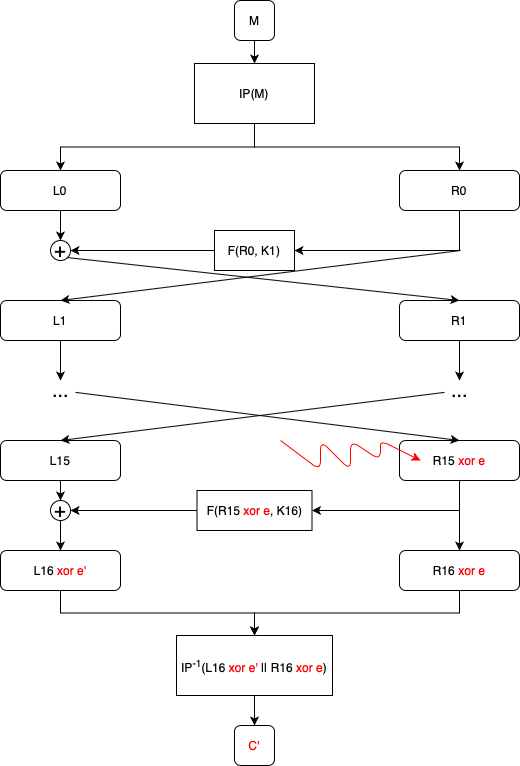
\includegraphics[scale=0.8]{../schemas/Schema_DES_attaque_faute.png}
\vspace*{\stretch{1}} \end{center}

\newpage
\subsection{Schéma de la génération des clés}
\label{schema 3}
\vspace*{\stretch{1}} \begin{center}
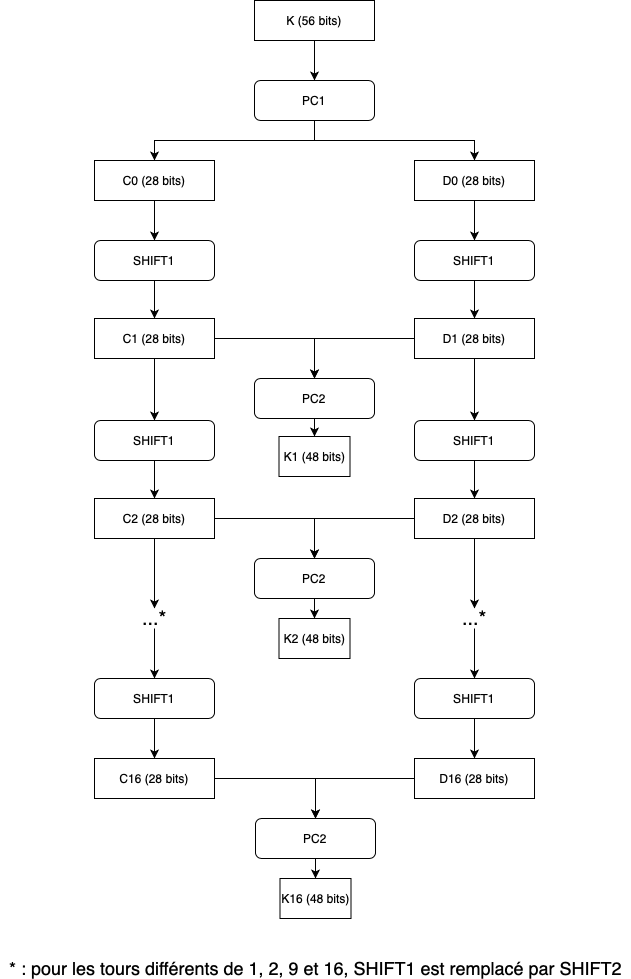
\includegraphics[scale=0.7]{../schemas/Schema_DES_generation_cles.png}
\vspace*{\stretch{1}} \end{center}

\end{document}
